\chapter{Interface Design}
\section{UX Diagram}
This diagram describes in detail all the pages of the application, how the application can
be navigated including the screens, the input forms and the possible errors.\\

\begin{figure}[!ht]
    \centering
	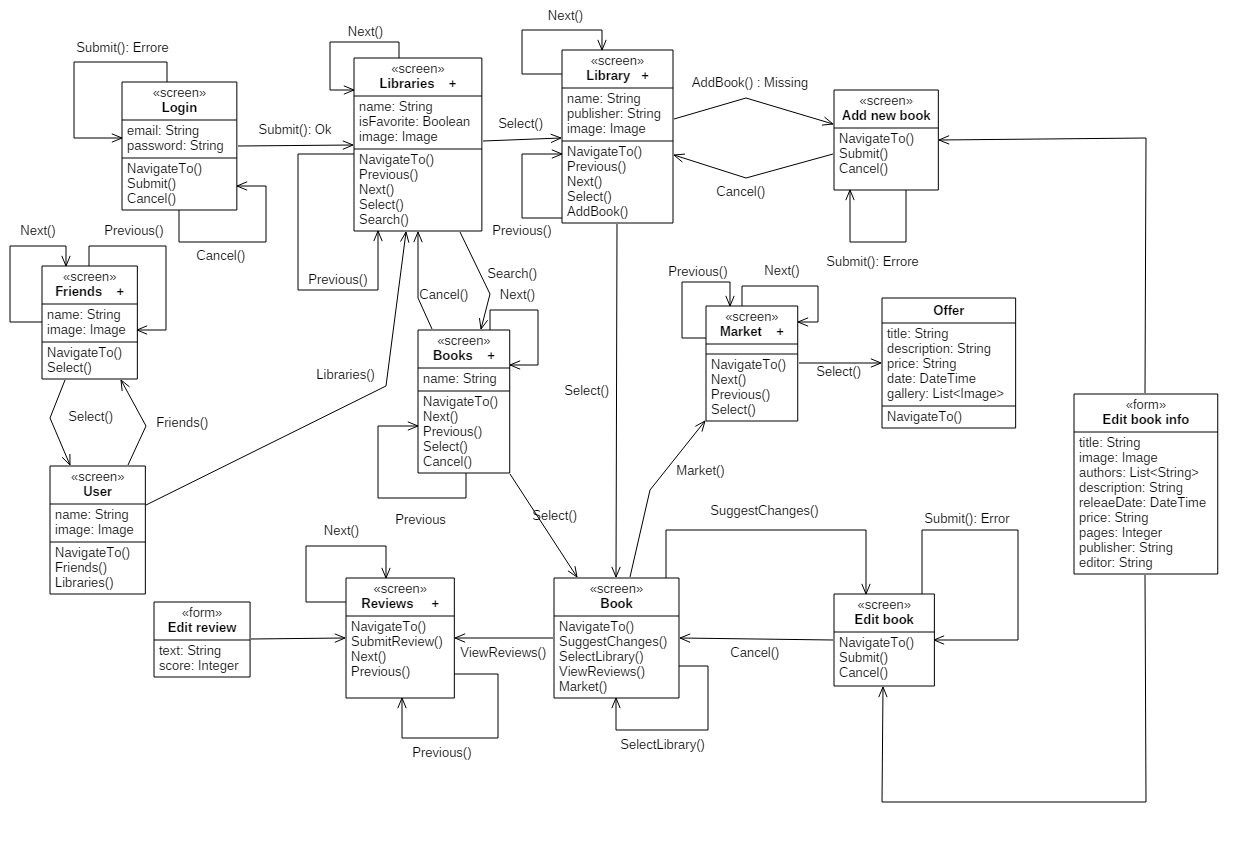
\includegraphics[scale=0.39]{images/ux-diagram.png}
	\caption{UX diagram}
	\label{fig:uxdiagram}
\end{figure}
\clearpage
\section{User Interfaces Design}
\section{Hardware Interfaces}
This project doesn’t require any hardware interface.
\section{Software Interfaces}
\begin{itemize}
    \item Database Management System (DBMS):
    \begin{itemize}
        \item 
        Name: Cloud Firestore
        \item 
        Source: https://firebase.google.com/products/firestore/
    \end{itemize}
    \item Storage:
    \begin{itemize}
        \item 
        Name: Cloud Storage
        \item 
        Source: https://firebase.google.com/products/storage
    \end{itemize}
    \item Server:
    \begin{itemize}
        \item 
        Name: Cloud Functions
        \item 
        Source: https://firebase.google.com/products/functions/
    \end{itemize}
    \item
    Operiting systems:
    \begin{itemize}
        \item 
        Name: Android
        \item 
        Minimum version: 5.0 Lollipop 
        \item 
        API level: 21
        \item 
        Source: https://www.android.com/\\ 
        \item 
        Name: iOS
        \item 
        Minimum version: 10
        \item 
        Source: https://www.apple.com/ios
    \end{itemize}
\end{itemize}
\section{API Interfaces}
The application communicates with the database on Firebase using:
\begin{itemize}
    \item
    firebase\_core (version 0.4.0+8), a Flutter plugin to use the Firebase Core API, which enables connecting to multiple Firebase apps.
    \item
    firebase\_analytics (version 4.0.2), allows to use the Google Analytics for Firebase API, a free app measurement solution that provides insight on app usage and user engagement.
    \item
    firebase\_auth (version 0.14.0), a plugin to use the Firebase Authentication API, that aims to make building secure authentication systems easy, while improving the sign-in and onboarding experience for end users. It provides an end-to-end identity solution, supporting email and password accounts, phone auth, and Google, Twitter, Facebook, and GitHub login, and more.
    \item
    cloud\_firestore (version 0.12.9), a library that allows to communicates with the NoSQL cloud database of Google (Firestore).
    \item
    firebase\_storage (version 3.0.5), a Flutter plugin to use the Cloud Storage API. Cloud Storage is used to upload images or other files on Firebase.
\end{itemize}
During the adding new book phase, the ISBN is read using the barcode, that allowed by flutter\_barcode\_scanner (version 0.1.5+1).
\\
\\
For the user's login, the system uses the Google Sign In API. This API provides the authentication of the user and retrives his main information (name and email).
The used libraries are google\_sign\_in (version 4.0.6) and firebase\_auth.
\\
\\
The plugins intl (version 0.15.8) and intl\_translation (version 0.17.3) are used to generate and manage the language of the application, according to the language of the OS.